\section{Introduction}

Let's consider the constant process $v(t,s)=v(s)$. 
In this scenario, once we determine the value of the experiment $v(s)$, we can derive the value of $v(t,s)$ for all time instants since its value remains unchanged.
This process is perfectly predictable.

In contrast, white noise is the opposite: it is a completely unpredictable process. 

Other processes lie between these two extremes.
Consequently, we can decompose a process into two parts: one purely deterministic and one purely non-deterministic:
\[v(t)=\tilde{v}(t)+\widehat{v}(t)\]
For $\tilde{v}(t)$, the knowledge of the past is sufficient to predict a value at a certain instant.
Note that $\tilde{v}(t)$ and $\widehat{v}(t)$ are independent: 
\[\mathbb{E}\left[ \tilde{v}(t_1)\widehat{v}(t_2) \right]=\mathbb{E}\left[ \tilde{v}(t_1)\right]\underbrace{\mathbb{E}\left[\widehat{v}(t_2) \right]}_0 =0\]
The correlation is given by:
\begin{align*}
    \tilde{\gamma}_v(\tau)  &=\mathbb{E}\left[v(t)v(t+\tau)\right] \\
                            &=\mathbb{E}\left[\left(\tilde{v}(t)+\widehat{v}(t)\right)\left(\tilde{v}(t+\tau)+\widehat{v}(t+\tau)\right)\right] \\
                            &=\mathbb{E}\left[\tilde{v}(t)+\tilde{v}(t+\tau)\right]\mathbb{E}\left[\widehat{v}(t)+\widehat{v}(t+\tau)\right] \\
                            &=\tilde{\gamma}_{\tilde{v}}(\tau)+\tilde{\gamma}_{\widehat{v}}(\tau)
\end{align*}

The purely nondeterministic component can be expressed as:
\[\widehat{v}(t)=\sum_{i=-\infty}^{t}W(t,1)\eta(i)=\sum_{i=-\infty}^{t}W(t-1)\eta(i)=\sum_{k=0}^\infty W(k)\eta(t-k)\]
Here, $\eta(\cdot) \sim WN(0,\lambda^2)$. 
This formula can be expanded as:
\begin{align*}
\widehat{v}(t)  &= W(0)\eta(t) + W(1)\eta(t-1) + W(2)\eta(t-2) + \dots \\
                &= W(0)\eta(t) + W(1)z^{-1}\eta(t) + W(2)z^{-2}\eta(t) + \dots \\
                &= \underbrace{\left(W(0) + W(1)z^{-1} + W(2)z^{-2} + \dots\right)}_{\text{transfer function }W(z)} \eta(t)  \\
\end{align*}
The stability of this function $W(z)$ implies the stationarity of the process $\widehat{v}(t)$.
\begin{figure}[H]
    \centering
    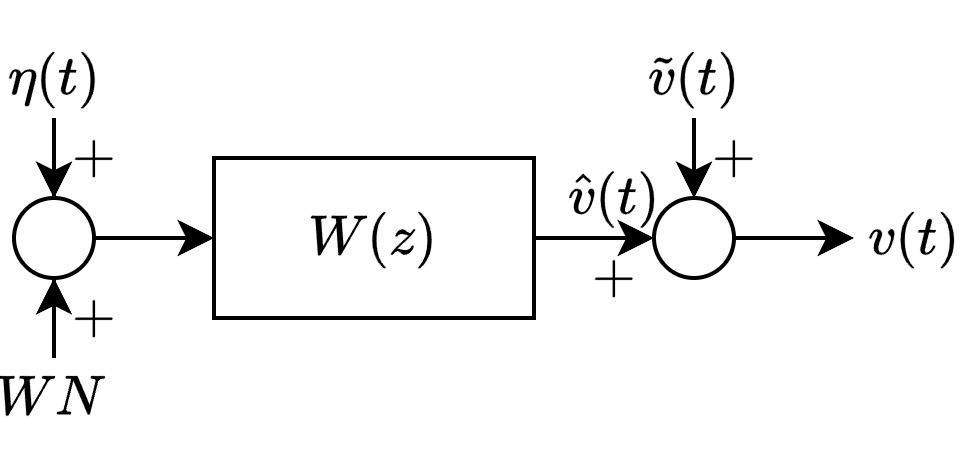
\includegraphics[width=0.4\linewidth]{images/dynamic.png} 
    \caption{Stochastic process composition}
\end{figure}